\section*{\underline{Aufgabe 19}}

\subsection*{a)}

Das ANFIS-Modell hat genau wie das Modell aus Aufgabe 18 vier Regeln.

\hfill

% train error: 0.39521
% check error: 0.44638

Der Fehler für die Trainingsdaten beträgt $0.39521$. Der Fehler für die Checking-Daten ist mit $0.44638$ etwas höher.

Beim in Aufgabe 18 generierten Modell lagen diese Werte bei $0.5276$ für die Trainingsdaten und bei $0.5856$ für die Checking-Daten.
Also ist das ANFIS Model in beider Hinsicht besser.

\subsection*{b)}

Dieses Modell besitzt 32 Regeln, gegenüber den nur vier Regeln aus a) und Aufgabe 18.

\hfill

% train error: 0.03301
% check error: 7.9124

Die Genauigkeit ist auf den ersten Blick viel besser als in a). Der Trainingsfehler beträgt nur $0.03301$. Sieht man sich die Visualisierung an, kann man sich aber denken, dass die Übereinstimmungen wahrscheinlich etwas zu präzise sind und das Modell starkes Overfitting aufweist, sich also exakt auf die Trainingsdaten eingestellt hat:

\hfill

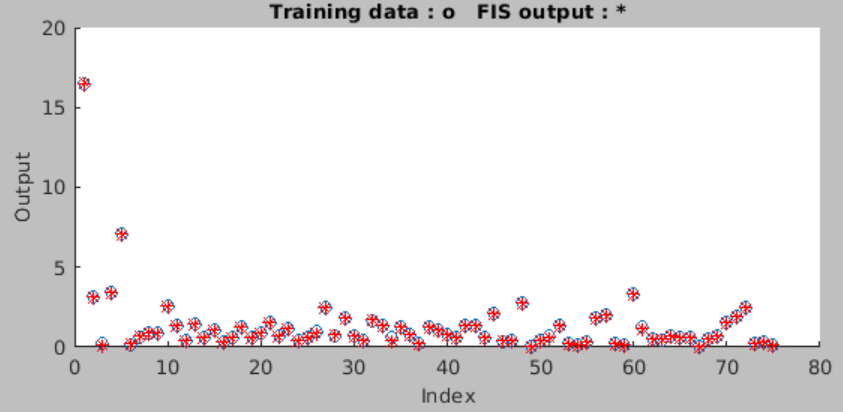
\includegraphics[width=\textwidth]{part/grid_train.png}

\hfill

Und tatsächlich beträgt der Fehler auf den Checking-Daten $7.9124$ gegenüber dem viel kleineren Fehler von $0.44638$ in a).

Gegen über Aufgabe 18 ist dies eine deutliche Regression für die Checking-Daten. 


\subsection*{c)}

	\textit{b) ANFID mit subtractive clustering} scheint am besten geeignet zu sein.
	
	\textit{a) genfis2 mit subtractive clustering)} liefert auch ein akzeptables Ergebnis wenn mit etwas mehr Fehler für sowohl Trainings-Daten als auch Checking-Daten im Verhältnis zu b).
	
	\textit{c) ANFIS mit grid partition} scheint sich hier nicht zu eignen da es zu deutlichem Overfitting kommt.
	
	\hfill
	
	Die Dritte Methode ist dann nicht geeignet, wenn die Trainings-Daten die Check-Daten bzw. die Realität nicht ausreichend repräsentieren. Da dann das Model sich zu sehr dan Trainings-Daten anpassen kann und sich dabei zu weit von der Realität entfernt das es dort nicht mehr nützlich ist.